\subsection{GPU Accelerating \textit{k}mer Counting}
While different GPU accelerated \textit{k}mer counting solutions such as Gerbil \cite{gerbil} have been developed in previous work, we opted to develop our own \textit{k}mer counting method because the \textit{k}mer counting problem solved in KAGE is slightly different than the typical \textit{k}mer counting problem described in section \ref{background:kmers_and_the_kmer_counting_problem}.
Rather than counting the frequency of every observed \textit{k}mer in the input reads, or even the frequency of every observed \textit{k}mer where the frequency is larger than some threshold, KAGE is only interested in counting the observed frequencies for a predetermined set of \textit{k}mers.
This revised problem is easier to solve in practice because the memory constraints are significantly less.
In the interest of brevity, we will refer to the typical \textit{k}mer counting problem described section \ref{background:kmers_and_the_kmer_counting_problem} as \textit{full kmer counting}, and the simpler problem where we only count the frequencies of a predetermined set of \textit{k}mers as \textit{partial kmer counting} \ref{methods:gpu_accelerating_kmer_counting:partial_kmer_counting}.

\definecolor{kmer1}{RGB}{40,40,215}
\definecolor{kmer2}{RGB}{0,150,0}
\definecolor{kmer3}{RGB}{225,30,30}
\definecolor{kmer4}{RGB}{20,150,150}

\begin{figure}[H]
\begin{center}
\scalebox{1}{
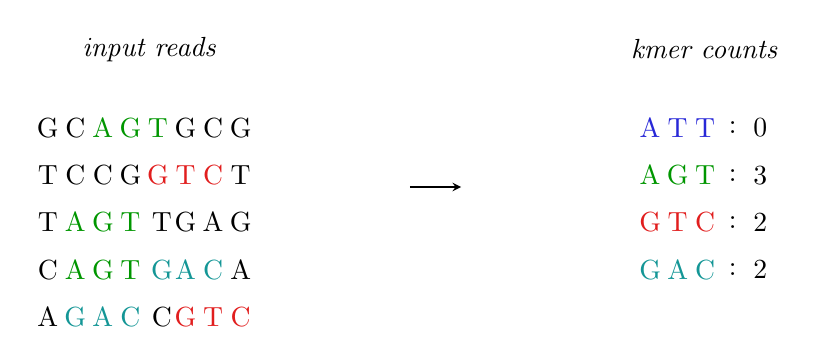
\begin{tikzpicture}
  % titles
  \node at(-0.55,3)(){\textit{input reads}};
  % read 1
  \node at(-1.85,2){G};
  \node at(-1.5,2){C};
  \node at(-1.15,2){\textcolor{kmer2}{A}};
  \node at(-.8,2){\textcolor{kmer2}{G}};
  \node at(-.45,2){\textcolor{kmer2}{T}};
  \node at(-.1,2){G};
  \node at(.25,2){C};
  \node at(.6,2){G};
  % read 2 
  \node at(-1.85,1.4){T};
  \node at(-1.5,1.4){C};
  \node at(-1.15,1.4){C};
  \node at(-.8,1.4){G};
  \node at(-.45,1.4){\textcolor{kmer3}{G}};
  \node at(-.1,1.4){\textcolor{kmer3}{T}};
  \node at(0.25,1.4){\textcolor{kmer3}{C}};
  \node at(.6,1.4){T};
  % read 3 
  \node at(-1.85,0.8){T};
  \node at(-1.5,0.8){\textcolor{kmer2}{A}};
  \node at(-1.15,0.8){\textcolor{kmer2}{G}};
  \node at(-.8,0.8){\textcolor{kmer2}{T}};
  \node at(-.4,0.8){T};
  \node at(-.1,0.8){G};
  \node at(.25,0.8){A};
  \node at(.6,0.8){G};
  % read 4 
  \node at(-1.85,0.2){C};
  \node at(-1.5,0.2){\textcolor{kmer2}{A}};
  \node at(-1.15,0.2){\textcolor{kmer2}{G}};
  \node at(-.8,0.2){\textcolor{kmer2}{T}};
  \node at(-.4,0.2){\textcolor{kmer4}{G}};
  \node at(-.1,0.2){\textcolor{kmer4}{A}};
  \node at(.25,0.2){\textcolor{kmer4}{C}};
  \node at(.6,0.2){A};
  % read 5 
  \node at(-1.85,-0.4){A};
  \node at(-1.5,-0.4){\textcolor{kmer4}{G}};
  \node at(-1.15,-0.4){\textcolor{kmer4}{A}};
  \node at(-.8,-0.4){\textcolor{kmer4}{C}};
  \node at(-.4,-0.4){C};
  \node at(-.1,-0.4){\textcolor{kmer3}{G}};
  \node at(.25,-0.4){\textcolor{kmer3}{T}};
  \node at(.6,-0.4){\textcolor{kmer3}{C}};
  % Arrow
  \draw [-stealth](2.75,1.25) -- (3.4,1.25);
  % k-mer counts
  \node at(6.5,3)(){\textit{kmer counts}};
  % k-mer 1
  \node at(5.8,2){\textcolor{kmer1}{A}};
  \node at(6.15,2){\textcolor{kmer1}{T}};
  \node at(6.5,2){\textcolor{kmer1}{T}};
  \node at(6.85,2){:};
  \node at(7.2,2){0};
  % k-mer 2 
  \node at(5.8,1.4){\textcolor{kmer2}{A}};
  \node at(6.15,1.4){\textcolor{kmer2}{G}};
  \node at(6.5,1.4){\textcolor{kmer2}{T}};
  \node at(6.85,1.4){:};
  \node at(7.2,1.4){3};
  % k-mer 3 
  \node at(5.8,0.8){\textcolor{kmer3}{G}};
  \node at(6.15,0.8){\textcolor{kmer3}{T}};
  \node at(6.5,0.8){\textcolor{kmer3}{C}};
  \node at(6.85,0.8){:};
  \node at(7.2,0.8){2};
  % k-mer 4 
  \node at(5.8,0.2){\textcolor{kmer4}{G}};
  \node at(6.15,0.2){\textcolor{kmer4}{A}};
  \node at(6.5,0.2){\textcolor{kmer4}{C}};
  \node at(6.85,0.2){:};
  \node at(7.2,0.2){2};
\end{tikzpicture}
}
\caption{
  In KAGE, we are only interested in counting the observed frequencies of a predefined set of \textit{k}mers, as opposed to every observed \textit{k}mer in the sequenced reads.
}
\label{methods:gpu_accelerating_kmer_counting:partial_kmer_counting}
\end{center}
\end{figure}
